\section{Section three}\label{sec:section3}

Reference to Figure~\ref{fig:plot}.

\begin{figure}[hbt!]
  \centering
  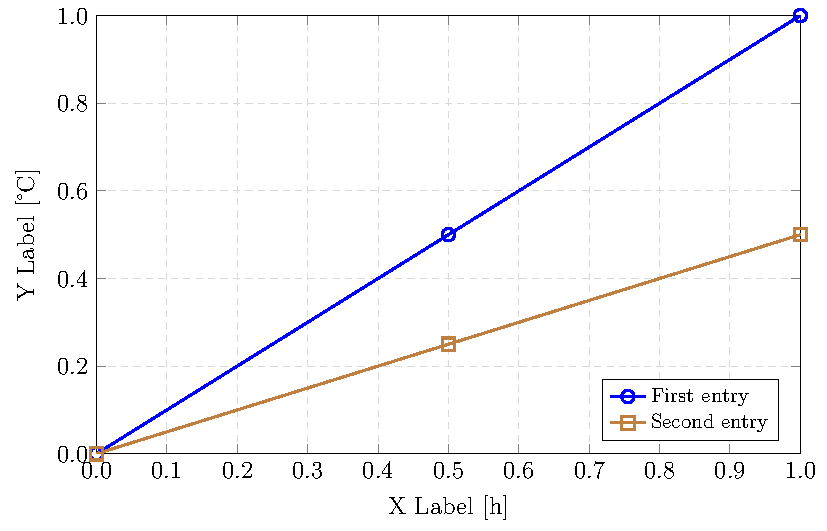
\includegraphics[width=0.8\linewidth]{figures/plot1.pdf}
  \caption{Figure caption}\label{fig:plot}
\end{figure}

This is a reference to Figure~\ref{fig:subfig}, which is divided into
Figure~\ref{fig:subfig-a} and Figure~\ref{fig:subfig-b}.

\begin{figure}[hbt!]
  \centering
  \begin{subfigure}[c]{0.49\textwidth}
    \centering
    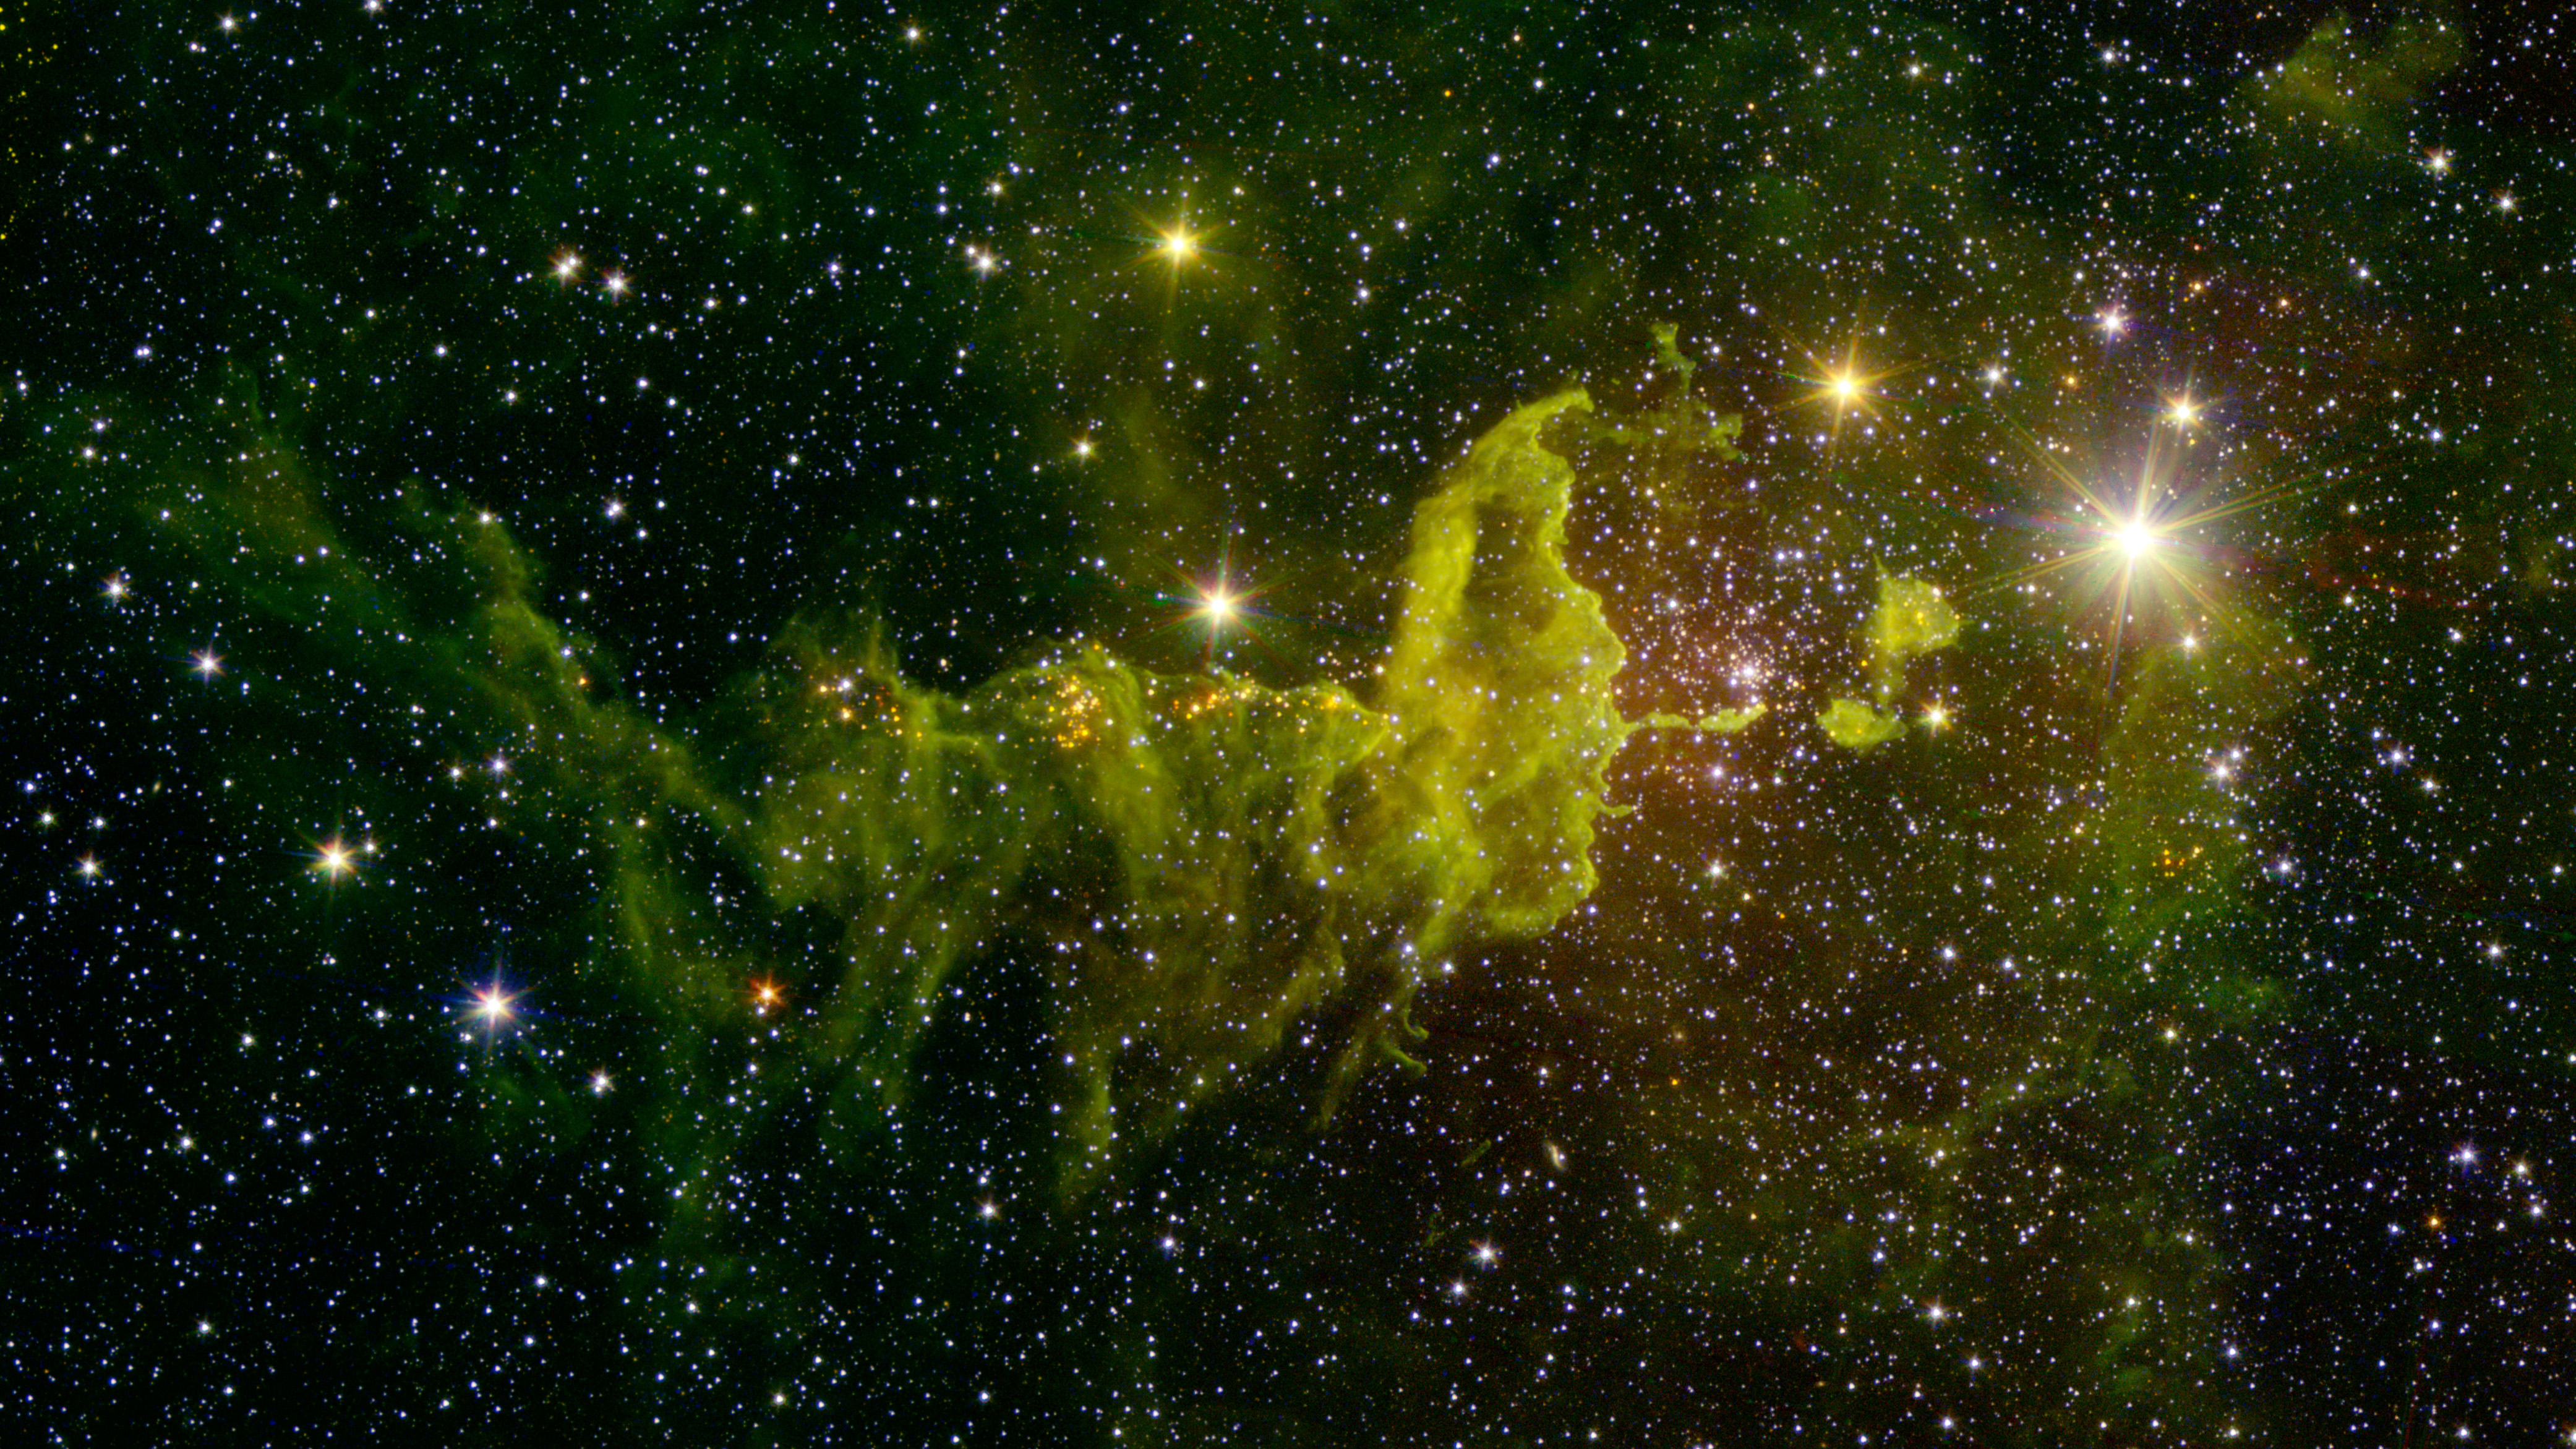
\includegraphics[width=\linewidth]{figures/figure1.jpg}
    \caption{}\label{fig:subfig-a}
  \end{subfigure}
  \begin{subfigure}[c]{0.49\textwidth}
    \centering
    
\includegraphics[width=\linewidth]{figures/figure2.jpg}
    \caption{}\label{fig:subfig-b}
  \end{subfigure}
  \caption{Figure with subfigures}\label{fig:subfig}
\end{figure}

Reference to Table~\ref{tab:table}.

\begin{table}[hbt!]
  \centering
  \renewcommand{\arraystretch}{1.1}
  \caption{Table caption}
  \begin{tabular}{p{0.3\linewidth}c{0.12\linewidth}c{0.12\linewidth}}
   \toprule
   \textbf{Column 1} & \textbf{Column 2} & \textbf{Column 3} \\
   \midrule
   Description 1 & 0.1 & 1.0 \\
   Description 2 & 0.2 & 2.0 \\
  \bottomrule
  \end{tabular}\label{tab:table}
  \renewcommand{\arraystretch}{1}
\end{table}

Reference to Equation~\ref{eq:relativity}.

\begin{equation}
\label{eq:relativity}
   E = mc^{2}
\end{equation}
